
%(BEGIN_QUESTION)
% Copyright 2015, Tony R. Kuphaldt, released under the Creative Commons Attribution License (v 1.0)
% This means you may do almost anything with this work of mine, so long as you give me proper credit

Calculate the amount of liquid lost from the vessel between 4:30 PM and 5:30 PM based on the information shown here:

$$\includegraphics[width=15.5cm]{i02888x01.eps}$$

$V_{lost}$ between 4:30 PM and 5:30 PM = \underbar{\hskip 50pt} gallons

\vskip 10pt

\underbar{file i02888}
%(END_QUESTION)





%(BEGIN_ANSWER)

This question is designed to probe your critical thinking, because there is absolutely no calculus involved in the answer!  Level transmitter LT-31 already measures the amount of liquid stored in the vessel, so calculating volume lost between any two points in time is simply a matter of subtracting those LT-31 values at those times:

$$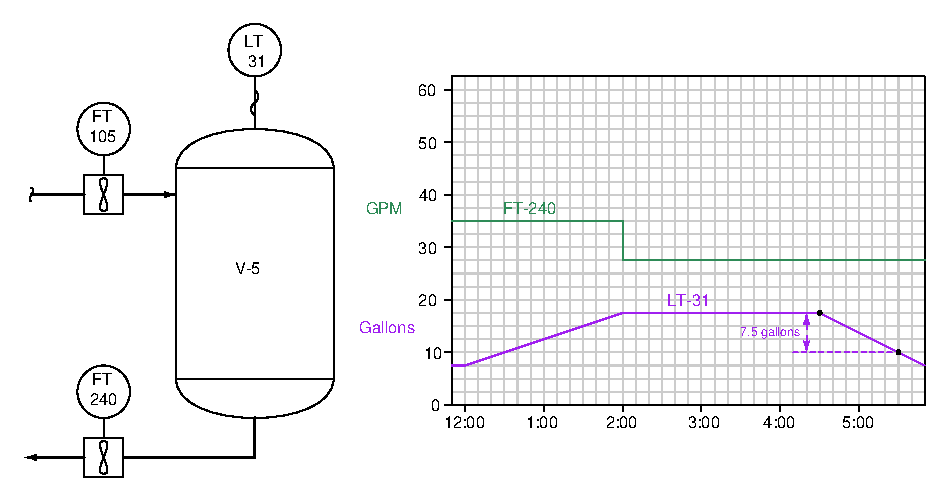
\includegraphics[width=15.5cm]{i02888x02.eps}$$

Since the vessel holds 17.5 gallons of liquid at 4:30 PM and holds 10 gallons of liquid at 5:30 PM, the amount of liquid lost from the vessel between those times is 7.5 gallons:

\vskip 10pt

$V_{lost}$ between 4:30 PM and 5:30 PM = \underbar{\bf 7.5} gallons

%(END_ANSWER)





%(BEGIN_NOTES)


%INDEX% Mathematics, calculus: integral (accumulated volume as the integral of flow)
%INDEX% Mathematics, calculus: integration (numerical)

%(END_NOTES)


